\documentclass{article} % For LaTeX2e
\usepackage{nips15submit_e,times}
\usepackage{hyperref}
\usepackage{url}
%\documentstyle[nips14submit_09,times,art10]{article} % For LaTeX 2.09

\usepackage{amsmath}
\usepackage{graphicx}
\usepackage{listings}             % Include the listings-package
\lstset{language=Python}          % Set your language (you can change the language for each code-block optionally)

\title{CSE253 Homework 2}


\author{
David S.~Hippocampus\\
Department of Computer Science\\
Cranberry-Lemon University\\
Pittsburgh, PA 15213 \\
\texttt{hippo@cs.cranberry-lemon.edu}
}

% The \author macro works with any number of authors. There are two commands
% used to separate the names and addresses of multiple authors: \And and \AND.
%
% Using \And between authors leaves it to \LaTeX{} to determine where to break
% the lines. Using \AND forces a linebreak at that point. So, if \LaTeX{}
% puts 3 of 4 authors names on the first line, and the last on the second
% line, try using \AND instead of \And before the third author name.

\newcommand{\fix}{\marginpar{FIX}}
\newcommand{\new}{\marginpar{NEW}}

%\nipsfinalcopy % Uncomment for camera-ready version

\begin{document}


\maketitle


\section{Problems I}


By the independence assumption on the $\epsilon^{i}$, we have the following likelihood function:



\begin{equation}
    \begin{array}{rcl}
       L(\theta) & = &  \prod\limits_{i = 1}^{m} p(y^{i} | x^{i} ; \theta)  \\
       & = &  \prod\limits_{i = 1}^{m} \frac{1}{\sqrt{2\pi} \sigma} exp(- \frac{(y^{(i)}   -   \theta^Tx^{(i)}  ) ^ 2}{2\sigma^2})
    \end{array}
\end{equation}

we should choose θ to maximize $L(\theta)$, it is same to maximize following function :

\begin{equation}
    \begin{array}{rcl}
       \ell(\theta) & = & \log{L(\theta)} \\
       & = &  \log {(\prod\limits_{i = 1}^{m} \frac{1}{\sqrt{2\pi} \sigma} exp(- \frac{(y^{(i)}   -   \theta^Tx^{(i)}  ) ^ 2}{2\sigma^2}))} \\
       & = & \sum\limits_{i = 1}^{m} \log {(\frac{1}{\sqrt{2\pi} \sigma} exp(- \frac{(y^{(i)}   -   \theta^Tx^{(i)}  ) ^ 2}{2\sigma^2}))} \\
       & = & m \log{ \frac{1}{\sqrt{2\pi} \sigma}  } - \frac{1}{\sigma^2} \cdot \frac{1}{2} \sum\limits_{i=1}^{m}(   y^{(i)}   -   \theta^Tx^{(i)}   )^2
    \end{array}
\end{equation}

Hence, maximizing $\ell(\theta)$ gives the same answer as minimizing \\

\begin{equation}
    \begin{array}{rcl}
       \frac{1}{2} \sum\limits_{i=1}^{m}(   y^{(i)}   -   \theta^Tx^{(i)}   )^2
    \end{array}
\end{equation}

So, we can conclude that finding the optimal parameter $\theta$ for the above linear regression problem on the dataset $D = \{  (x^{1},t^{1}), ... , (x^{(N)},t^{(N)})  \}$ is equal to finding the $\theta$ that minimizes the SSE:
\begin{equation}
    \begin{array}{rcl}
       \theta^* & = & argmin_\theta \sum\limits_{i=1}^{N}(  t^i - f((1,x^{(i)}), \theta) )^2
    \end{array}
\end{equation}



%% \subsection{Double-blind reviewing}

%% This year we are doing double-blind reviewing: the reviewers will not know 
%% who the authors of the paper are. For submission, the NIPS style file will 
%% automatically anonymize the author list at the beginning of the paper.

%% Please write your paper in such a way to preserve anonymity. Refer to
%% previous work by the author(s) in the third person, rather than first
%% person. Do not provide Web links to supporting material at an identifiable
%% web site.

%%\subsection{Electronic submission}
%%
%% \textbf{THE SUBMISSION DEADLINE IS June 5, 2015. SUBMISSIONS MUST BE LOGGED BY
%% 23:00, June 5, 2015, UNIVERSAL TIME}

%% You must enter your submission in the electronic submission form available at
%% the NIPS website listed above. You will be asked to enter paper title, name of
%% all authors, keyword(s), and data about the contact
%% author (name, full address, telephone, fax, and email). You will need to
%% upload an electronic (postscript or pdf) version of your paper.

%% You can upload more than one version of your paper, until the
%% submission deadline. We strongly recommended uploading your paper in
%% advance of the deadline, so you can avoid last-minute server congestion.
%%
%% Note that your submission is only valid if you get an e-mail
%% confirmation from the server. If you do not get such an e-mail, please
%% try uploading again. 

\section{Problems II}

(a) \\

\begin{equation}
    \begin{array}{rcl}
      	 \delta_k & = & - \frac{\partial{E}}{\partial{a_k}} \\
	 & = & - \frac{\partial{E}}{\partial{\tilde{g}(a_k)}} \frac{\partial{\tilde{g}(a_k)}} {\partial{a_k}} \\
	 & = & \frac{(y_k - t_k)}{\tilde{g}'(a_k)} \\
	 & = & (t_k - y_k)
    \end{array}
\end{equation}


\begin{equation}
    \begin{array}{rcl}
      	 \delta_j & = & - \frac{\partial{E}}{\partial{a_j}} \\
	 & = & - \sum\limits_{k=1}^{c} \frac{\partial{E}}{\partial{a_k}} \frac{\partial{a_k}}{\partial{a_j}} \\
	 & = & - \sum\limits_{k=1}^{c} \frac{\partial{E}}{\partial{a_k}} \frac{\partial{a_k}}{\partial{z_j}} \frac{\partial{z_j}}{\partial{a_j}} \\
	 & = & g'(a_j) \sum\limits_{k=1}^{c}  \delta_k w_{jk}
    \end{array}
\end{equation}

(b) \\

\begin{equation}
    \begin{array}{rcl}
      	 w_{jk}(t+1) & = & w_{jk}(t) - \alpha \frac{\partial{E}}{\partial{w_{jk}(t)}} \\
	 & = & w_{jk}(t) - \alpha \frac{\partial{E}}{\partial{a_k}}z_j \\
	 & = & w_{jk}(t) + \alpha \delta_k z_j
    \end{array}
\end{equation}

\begin{equation}
    \begin{array}{rcl}
      	 w_{ij}(t+1) & = & w_{ij}(t) - \alpha \frac{\partial{E}}{\partial{w_{ij}}} \\
	 & = & w_{ij}(t) - \alpha \frac{\partial{E}}{\partial{a_j}}   \frac{\partial{a_j}}{\partial{w_{ij}}} \\
	 & = & w_{ij}(t) + \alpha  \delta_j x_i
    \end{array}
\end{equation}

(c) \\
T is the target, Y is output. Assuming $Z : 1 \times \ell$

\begin{equation}
    \begin{array}{rcl}
      	 w_{HO} & = & w_{HO} + \alpha * ( (T - Y)^T \cdot Z) \\
	 w_{IH} & = & w_{IH} + \alpha X^T  \cdot (  Z * ( (1)_{1 \times \ell} - Z)   * (   (T - Y) \cdot W_{HO}^T )     )
    \end{array}
\end{equation}

(d) \\ i.
I use scipy to zscore raw data. \\

ii. The gradient using numerical differences with the one using backpropagation is very close. So my algorithm produce right gradient.

iii. First, I use Normal distribution with scale 0.1 to initialize parameters. Then I divide my data into 30 racks and run training on these racks individually instead of the total data. I also test different iteration numbers and different learning rate.

\begin{figure}[htbp] %  figure placement: here, top, bottom, or page
   \centering
   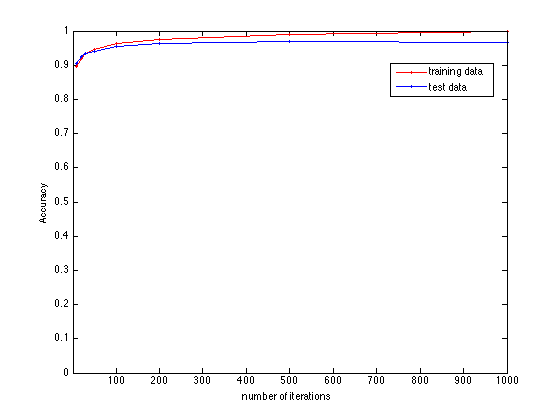
\includegraphics[width=5in]{img/p4.png} 
\end{figure}

\pagebreak

(e) \\
\begin{figure}[htbp] %  figure placement: here, top, bottom, or page
   \centering
   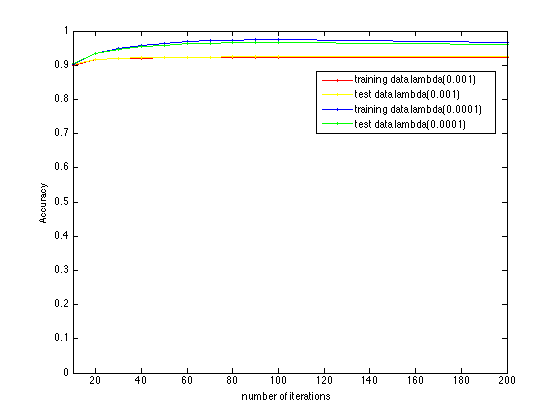
\includegraphics[width=5in]{img/p5.png} 
\end{figure}

\end{document}